
\section{Policy Learning for Swing-Up}


The objective of the control part is to learn policies that swing up the
unbalanced disk from the stable downward equilibrium and stabilize it around
the unstable upright position \cite{assignment5sc28,course5sc28}. The input is the motor voltage and is constrained
by
\begin{equation}
    u_k \in [-3,3]~\mathrm{V}.
\label{eq:policy_voltage_limit}
\end{equation}
The disk angle $\theta$ and angular velocity $\omega$ are used as full state
feedback. The downward position is defined as $\theta=0$, while the upright
target corresponds to $\theta=\pi$. Since the angle is periodic, the upright
error is evaluated using the wrapped angle error
\begin{equation}
    e_{\theta,k}=\mathrm{wrap}(\theta_k-\pi),
\label{eq:policy_upright_error}
\end{equation}
so that both $\theta=\pi$ and $\theta=-\pi$ represent the same physical upright
configuration.

Two learning-based controllers are considered. The first one is a Deep
Q-Network (DQN) controller, which represents the Q-learning-based part of the
assignment. It learns a discrete-action voltage policy from simulator
interaction by approximating the action-value function with a neural network
\cite{course5sc28,watkins1992qlearning,mnih2015dqn}.
The second controller is a hybrid energy-pumping and RBF-based policy
improvement method. In this approach, an energy-pumping law is used for the
global swing-up phase, while an RBF policy initialized from local PD supervision
is used for stabilization near the upright position and further improved by
simulator-based optimization \cite{course5sc28,broomhead1988rbf}.

The controllers are evaluated using rollout-based metrics, including final and
last-window wrapped angle error, upright ratio, input saturation ratio, and
multi-seed success rate. These metrics assess not only whether the disk reaches
the upright position, but also whether it remains stable there without excessive
voltage saturation. The following sections present the DQN controller, the
hybrid RBF controller, and their comparison.



\subsection{Control Objective and Evaluation Metrics}

The control objective is to swing up the disk from the downward stable position
to the upright unstable equilibrium and keep it stabilized around that position.
For policy learning, full state feedback is allowed, so the controller uses
\begin{equation}
    x_k =
    \begin{bmatrix}
        \theta_k \\
        \omega_k
    \end{bmatrix},
\label{eq:policy_full_state}
\end{equation}
where $\theta_k$ is the measured disk angle and $\omega_k$ is the angular
velocity. The motor voltage is constrained by
\begin{equation}
    u_k \in [-3,3]~\mathrm{V}.
\label{eq:policy_input_constraint}
\end{equation}

Since the disk angle is periodic, the upright error is defined as the wrapped
angle error
\begin{equation}
    e_{\theta,k} = \mathrm{wrap}(\theta_k-\pi),
\label{eq:policy_wrapped_error}
\end{equation}
so that both $\theta=\pi$ and $\theta=-\pi$ correspond to the same physical
upright configuration. A successful controller should make
$|e_{\theta,k}|$ small and reduce $|\omega_k|$ after the disk reaches the
upright region.

The controllers are evaluated using rollout-based metrics, including the final
wrapped angle error, the minimum absolute error, the mean absolute error over
the last $N_w=100$ time steps, the last-window angular velocity, the upright
ratio, and the input saturation ratio. The upright ratio measures how long the
disk remains close to the target, while the saturation ratio measures how often
the input reaches the voltage limits. For multi-seed robustness evaluation, a
rollout is considered successful if
\begin{equation}
\begin{aligned}
    e_{\mathrm{last}} < 0.10
    \quad \mathrm{and} \quad
    r_{\mathrm{upright}} > 0.70.
\end{aligned}
\label{eq:policy_success_condition}
\end{equation}
The success rate is then computed as the fraction of successful rollouts over
all tested seeds.



\subsubsection{Method and State-Action Representation}

The first learning-based controller was implemented using Deep Q-Network (DQN)
learning, which represents the Q-learning-based method in this project
\cite{watkins1992qlearning,mnih2015dqn}. Since
the disk angle and angular velocity are continuous variables, a tabular
Q-function is not practical. Therefore, a neural network was used to approximate
the action-value function \(Q(s_k,u_k)\). After training, the controller applies
the greedy action
\begin{equation}
    u_k = \arg\max_{u \in \mathcal{U}} Q(s_k,u).
\label{eq:dqn_greedy_action}
\end{equation}

The DQN state was defined as
\begin{equation}
    s_k =
    \begin{bmatrix}
        \sin\theta_k \\
        \cos\theta_k \\
        \omega_k/10
    \end{bmatrix}.
\label{eq:dqn_state}
\end{equation}
The sine-cosine representation avoids the discontinuity of the periodic angle
at \(\theta=\pm\pi\), while the angular velocity is scaled to keep all state
components in a similar numerical range.

Because DQN is a discrete-action method, the motor voltage was discretized as
\begin{equation}
    \mathcal{U} =
    \{-3,-2,-1,0,1,2,3\}~\mathrm{V}.
\label{eq:dqn_action_set}
\end{equation}
This action set satisfies the voltage constraint by construction. The DQN
network takes \(s_k\) as input and outputs one Q-value for each admissible
voltage action. During evaluation, the action with the highest Q-value is
applied to the simulator. The main advantage of this design is that it enables
Q-learning on the continuous-state unbalanced disk system, while the main
limitation is that the resulting voltage input is discrete and may be less
smooth than a continuous-action policy.


\subsubsection{Reward Function and Training Setup}

The DQN reward was shaped to encourage both energy injection during the
swing-up phase and stabilization near the upright position. A sparse reward
based only on the final upright condition would make exploration difficult, so
the reward was constructed from height, upright, bonus, angular-velocity, and
input-effort terms:
\begin{equation}
\begin{aligned}
    r_k =
    r_{\mathrm{height},k}
    + r_{\mathrm{upright},k}
    + r_{\mathrm{bonus},k}
    - r_{\omega,k}
    - r_{u,k}.
\end{aligned}
\label{eq:dqn_reward}
\end{equation}
The height term encourages the disk to move away from the downward equilibrium,
while the upright and bonus terms reward small wrapped error near the target.
The angular-velocity and input penalties reduce excessive oscillation and
unnecessary control effort. The stabilization-related terms use
\begin{equation}
    e_{\theta,k}=\mathrm{wrap}(\theta_k-\pi),
\label{eq:dqn_reward_error}
\end{equation}
so that both \(\theta=\pi\) and \(\theta=-\pi\) are treated as the same upright
configuration.

Training was performed in the official unbalanced-disk simulator using an
\(\epsilon\)-greedy exploration strategy \cite{course5sc28}. The exploration probability was
gradually reduced during training, so that the agent first explored different
swing-up behaviors and later relied more on the learned Q-function. Experience
replay and a target network were used to improve the stability of the DQN
updates \cite{mnih2015dqn}. The best checkpoint was selected based on the evaluation rollout
performance and was later tested using the greedy policy without exploration.

\begin{figure}[H]
    \centering
    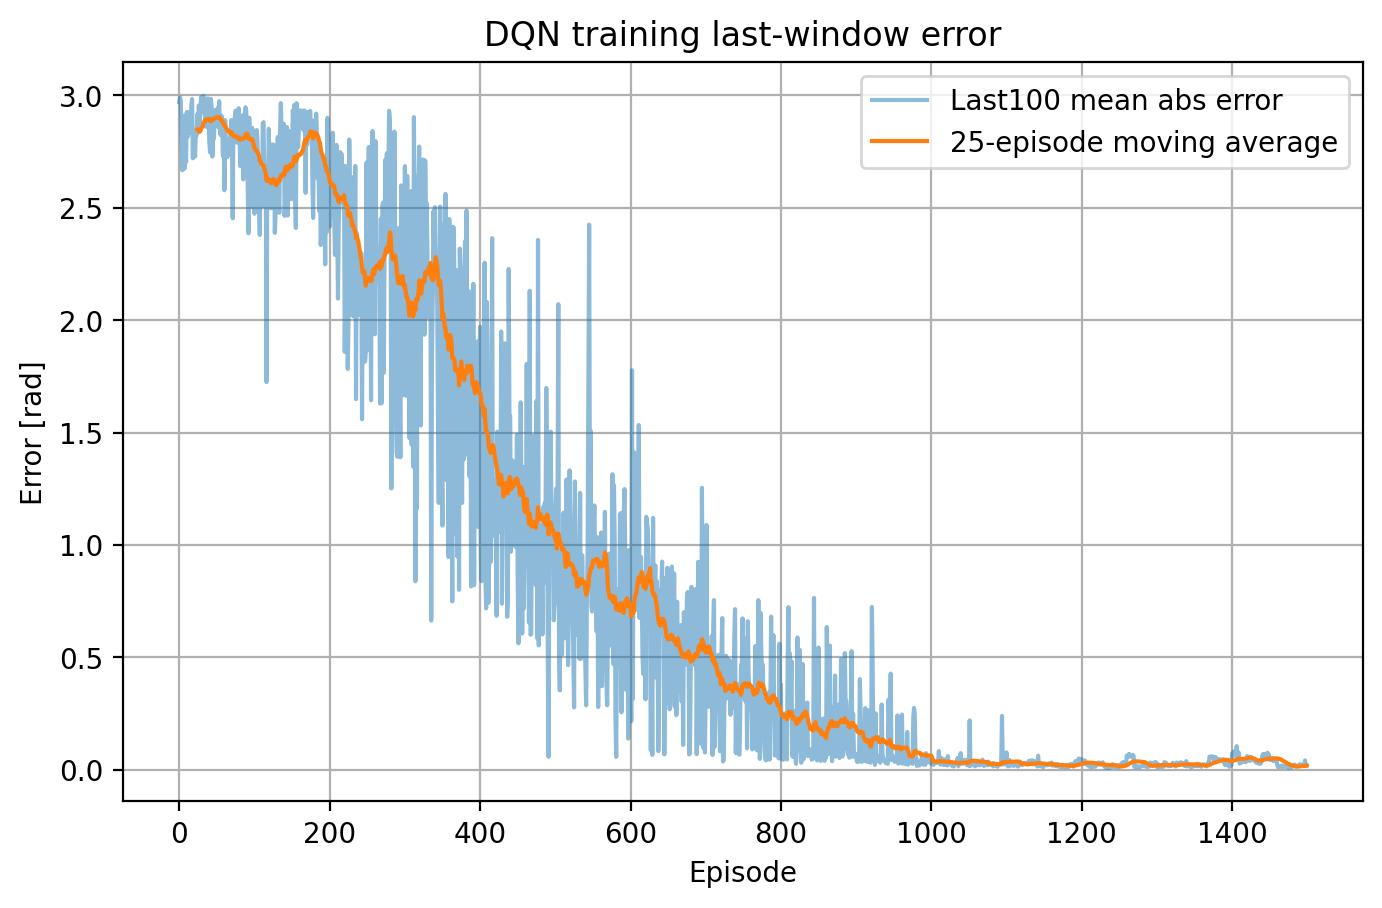
\includegraphics[width=0.85\linewidth]{figures/dqn_training_last100_error.png}
    \caption{Last-window mean absolute angle error during DQN training. The
    decreasing error indicates that the learned policy gradually improves its
    final upright stabilization performance.}
    \label{fig:dqn_training_error}
\end{figure}

As shown in Fig.~\ref{fig:dqn_training_error}, the training error decreases as
the agent collects more simulator experience. This confirms that the learned
Q-function gradually improves from random exploratory behavior to an effective
swing-up and stabilization policy.


\subsubsection{Simulation Results}

After training, the best DQN checkpoint was evaluated using the greedy policy
without exploration,
\begin{equation}
    u_k = \arg\max_{u \in \mathcal{U}} Q(s_k,u).
\label{eq:dqn_eval_action}
\end{equation}
Figure~\ref{fig:dqn_greedy} shows that the wrapped angle error decreases after
the swing-up phase and remains close to zero near the end of the rollout. This
confirms that the learned DQN policy can drive the disk to the upright
configuration and stabilize it there in simulation.

\begin{figure}[H]
    \centering
    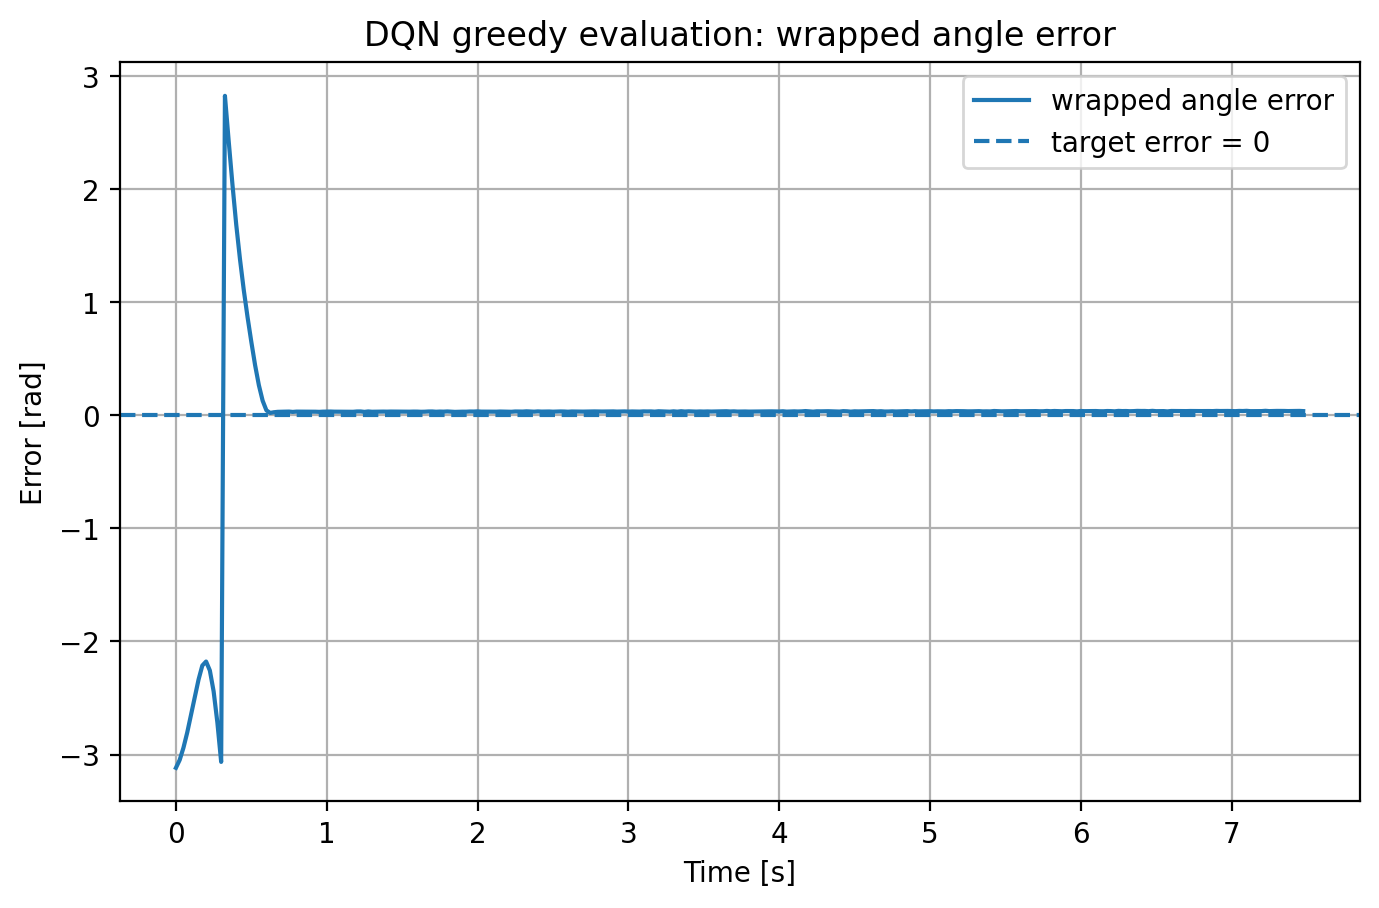
\includegraphics[width=0.85\linewidth]{figures/dqn_eval_best_error.png}
    \caption{Wrapped angle error of the greedy DQN policy. The error converges
    close to zero after the swing-up phase.}
    \label{fig:dqn_greedy}
\end{figure}

The best policy was further evaluated over 20 random simulation seeds. The
results in Table~\ref{tab:dqn_results} show that the DQN achieved a success
rate of $1.000$. The last-window mean absolute error was $0.0317$ rad and the
last-window mean absolute angular velocity was $0.0014$ rad/s, indicating that
the disk was stabilized near the upright position rather than only passing
through it.

\begin{table}[htbp]
    \caption{Multi-seed evaluation performance of the best DQN policy.}
    \centering
    \begin{tabular}{lc}
        \toprule
        Metric & Value \\
        \midrule
        Evaluation seeds & 20 \\
        Success rate & 1.000 \\
        Final error [rad] & $0.0326 \pm 0.0068$ \\
        Min. abs. error [rad] & $0.0198 \pm 0.0026$ \\
        Mean abs. error [rad] & $0.1879 \pm 0.0054$ \\
        Last-window error [rad] & $0.0317 \pm 0.0062$ \\
        Last-window $|\omega|$ [rad/s] & $0.0014 \pm 0.0014$ \\
        Upright ratio & $0.9233 \pm 0.0000$ \\
        Saturation ratio & $0.0733 \pm 0.0000$ \\
        Return & $1385.6200 \pm 1.5405$ \\
        \bottomrule
    \end{tabular}
    \label{tab:dqn_results}
\end{table}

Overall, the DQN controller successfully solved the swing-up and stabilization
task in simulation. Its main advantage is that it learns the control policy
directly from interaction data without an explicit analytical swing-up law.
However, the controller uses a discrete voltage action set, so the resulting
input may be less smooth than that of a continuous policy.



\subsection{Hybrid Energy-Pumping and RBF Policy Improvement}

\subsubsection{Design Motivation and Hybrid Policy Structure}

The second controller was developed as a hybrid energy-pumping and RBF-based
policy improvement method. In contrast to the DQN controller, which learns a
value function from simulator interaction, this approach combines physical
insight for the swing-up phase with a learned nonlinear local stabilizer near
the upright position \cite{course5sc28,broomhead1988rbf}. This controller is used as the model-internalization or
policy-improvement branch of the study.

A direct global RBF imitation policy was first tested using teacher data from
an energy-pumping and local PD controller. However, closed-loop simulations
showed that the global RBF policy was not robust: it could sometimes pass
through the upright region, but often failed to stabilize the disk or produced
nearly saturated inputs. Therefore, the task was separated into a global
swing-up part and a local stabilization part.

The resulting hybrid policy is
\begin{equation}
\begin{aligned}
    u_k =
    \begin{cases}
        u_{\mathrm{energy}}(\theta_k,\omega_k),
        & |e_{\theta,k}| \geq \epsilon, \\[2mm]
        g_{\mathrm{RBF}}\pi_{\mathrm{RBF}}(x_k),
        & |e_{\theta,k}| < \epsilon,
    \end{cases}
\end{aligned}
\label{eq:hybrid_policy}
\end{equation}
where \(e_{\theta,k}=\mathrm{wrap}(\theta_k-\pi)\), \(\epsilon\) is the
switching threshold, and \(g_{\mathrm{RBF}}\) is the local stabilizer gain. The
energy-pumping controller injects energy when the disk is far from the upright
position, while the RBF policy is only used near the target region.

The RBF stabilizer uses the local state
\begin{equation}
    x_k =
    \begin{bmatrix}
        e_{\theta,k} \\
        \omega_k
    \end{bmatrix}
\label{eq:hybrid_local_state}
\end{equation}
and is written as the saturated feedback law
\begin{equation}
    \pi_{\mathrm{RBF}}(x_k)
    =
    u_{\max}\tanh\!\left(\Phi(x_k)w\right),
\label{eq:rbf_policy}
\end{equation}
with \(u_{\max}=3\) V. The hyperbolic tangent bounds the RBF output, and the
final input is clipped to satisfy \(u_k\in[-3,3]\) V. This structure reduces the
learning difficulty because the RBF policy only needs to learn local upright
stabilization, while the analytical energy-pumping law handles the global
swing-up motion.


\subsubsection{RBF Local Stabilizer Initialization}

After selecting the hybrid structure, the RBF component was initialized as a
local stabilizer around the upright equilibrium. Instead of using complete
swing-up teacher trajectories, a local supervision dataset was generated from a
PD controller, because the RBF policy is only active near the upright position.
The local state was defined as
\begin{equation}
    x =
    \begin{bmatrix}
        e_\theta \\
        \omega
    \end{bmatrix},
\label{eq:rbf_training_state}
\end{equation}
and the supervision grid covered
\begin{equation}
\begin{aligned}
    e_\theta \in [-0.6,0.6],
    \qquad
    \omega \in [-8,8].
\end{aligned}
\label{eq:rbf_training_grid}
\end{equation}
For each grid point, the target input was computed using
\begin{equation}
\begin{aligned}
    u_{\mathrm{PD}} = -K_p e_\theta - K_d \omega,
    \qquad
    K_p=10.0,\quad K_d=1.5,
\end{aligned}
\label{eq:rbf_pd_target}
\end{equation}
and clipped to the admissible range \([-3,3]\) V.

The RBF policy was trained to reproduce this local PD behavior using the
saturated form
\begin{equation}
    \pi_{\mathrm{RBF}}(x)
    =
    u_{\max}\tanh\!\left(\Phi(x)w\right).
\label{eq:rbf_saturated_policy}
\end{equation}
The final local stabilizer used 121 RBF basis functions and 122 trainable
parameters including the bias term. On the local supervision grid, the mean
absolute input error was
\begin{equation}
    \mathrm{MAE}_u = 0.0571~\mathrm{V},
\label{eq:rbf_mae}
\end{equation}
which indicates that the RBF policy accurately approximates the desired local
PD stabilizing action.

The initialized RBF stabilizer was then combined with the analytical
energy-pumping controller. The initial switching threshold was set to
\(\epsilon=0.45\) rad. As shown in Fig.~\ref{fig:hybrid_initial_angle}, the
initialized hybrid controller successfully swung up the disk and stabilized it
near the upright configuration in simulation. This provided a suitable starting
point for the following simulator-based policy improvement step.

\begin{figure}[H]
    \centering
    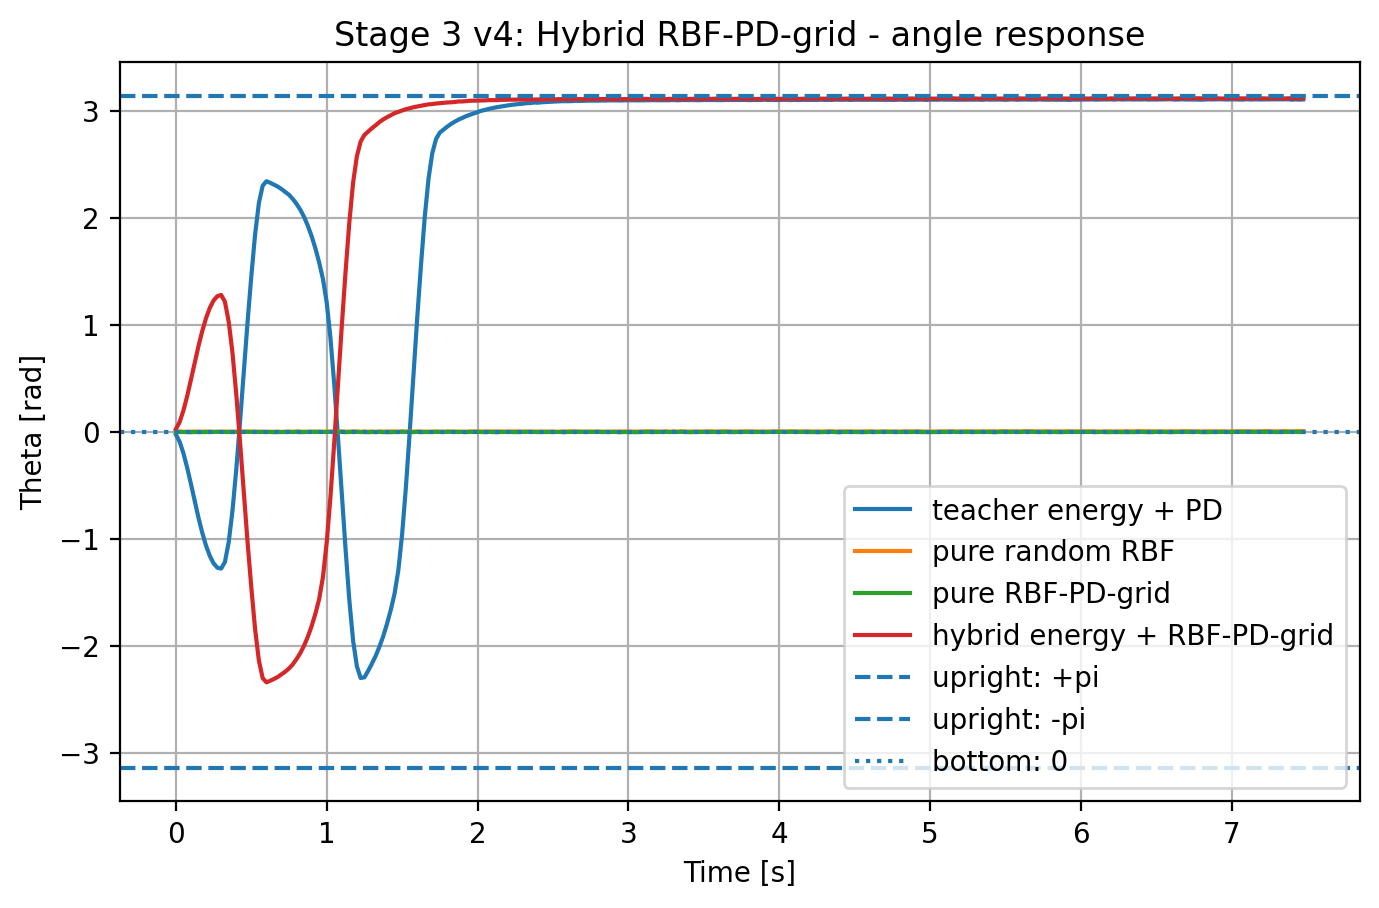
\includegraphics[width=0.85\linewidth]{figures/hybrid_rbf_pd_theta.png}
    \caption{Angle response of the initialized hybrid energy-pumping and
    RBF-PD-grid controller.}
    \label{fig:hybrid_initial_angle}
\end{figure}



\subsubsection{Simulator-Based Policy Improvement}

After the initialized hybrid controller achieved successful swing-up in
simulation, simulator-based policy improvement was applied to refine its
high-level behavior. Instead of optimizing all RBF weights, only four
hybrid-level parameters were tuned:
\begin{equation}
    p =
    \begin{bmatrix}
        \epsilon &
        g_{\mathrm{RBF}} &
        a_{\mathrm{energy}} &
        a_{\mathrm{kick}}
    \end{bmatrix}^{\top},
\label{eq:hybrid_parameters}
\end{equation}
where \(\epsilon\) is the switching threshold, \(g_{\mathrm{RBF}}\) is the RBF
stabilizer gain, \(a_{\mathrm{energy}}\) is the energy-pumping amplitude, and
\(a_{\mathrm{kick}}\) is the initial kick amplitude. This keeps the optimization
low-dimensional while preserving the PD-initialized RBF stabilizer.

The initial parameter vector was
\begin{equation}
    p_0 =
    \begin{bmatrix}
        0.45 & 1.00 & 3.00 & 2.50
    \end{bmatrix}^{\top}.
\label{eq:hybrid_initial_parameters}
\end{equation}
The parameters were optimized in the simulator using a rollout-based objective
that penalized final angle error, angular velocity, input effort, and input
saturation, while rewarding successful upright stabilization. Differential
evolution was used for global search, followed by Powell optimization for local
refinement \cite{storn1997differential,powell1964efficient}. The optimized parameter vector was
\begin{equation}
    p^{\star} =
    \begin{bmatrix}
        0.5785 & 1.3974 & 2.7481 & 2.3309
    \end{bmatrix}^{\top}.
\label{eq:hybrid_optimized_parameters}
\end{equation}
Compared with the initial controller, the optimized policy switches earlier to
the RBF stabilizer, applies a stronger local stabilizing gain, and uses smaller
energy-pumping and kick amplitudes. This improves stabilization accuracy while
reducing input saturation.

\begin{table}[htbp]
    \caption{Simulator-based policy optimization results for the hybrid
    controller.}
    \centering
    \begin{tabular}{lcc}
        \toprule
        Metric & Initial & Optimized \\
        \midrule
        Final error [rad] & $-0.025$ & $-0.011$ \\
        Min. abs. error [rad] & $0.021$ & $0.011$ \\
        Last-window error [rad] & $0.025$ & $0.013$ \\
        Saturation ratio & $0.233$ & $0.000$ \\
        Upright ratio & $0.753$ & $0.847$ \\
        RBF mode ratio & $0.767$ & $0.867$ \\
        \bottomrule
    \end{tabular}
    \label{tab:hybrid_optimization}
\end{table}

As shown in Table~\ref{tab:hybrid_optimization}, the optimized hybrid policy
reduced the last-window error from \(0.025\) rad to \(0.013\) rad and decreased
the saturation ratio from \(0.233\) to \(0.000\). Thus, the simulator-based
policy improvement made the controller more accurate and less dependent on
saturated voltage input.


\subsubsection{Robustness Evaluation}

The optimized hybrid policy was evaluated over 50 random simulation seeds to
test whether the controller generalizes to different initial perturbations and
stochastic simulation conditions. The controller parameters were fixed during
this evaluation, and no further training or optimization was performed. A
rollout was classified as successful if
\begin{equation}
\begin{aligned}
    e_{\mathrm{last}} < 0.10
    \quad \mathrm{and} \quad
    r_{\mathrm{upright}} > 0.70.
\end{aligned}
\label{eq:hybrid_success_condition}
\end{equation}

Table~\ref{tab:hybrid_robustness} summarizes the robustness results. The
optimized hybrid policy achieved a $100\%$ success rate over all 50 rollouts.
The mean last-window error was only $0.0129$ rad, and the last-window angular
velocity was $0.0011$ rad/s, indicating stable upright behavior rather than a
short pass through the target. The saturation ratio was zero for all rollouts,
and the maximum absolute input was $2.7481$ V, which remains below the
\(\pm 3\) V voltage limit.

\begin{table}[htbp]
    \caption{Robustness evaluation of the optimized hybrid policy over 50
    random seeds.}
    \centering
    \begin{tabular}{lc}
        \toprule
        Metric & Value \\
        \midrule
        Final error [rad] & $0.0010 \pm 0.0118$ \\
        Min. abs. error [rad] & $0.0099 \pm 0.0005$ \\
        Last-window error [rad] & $0.0129 \pm 0.0002$ \\
        Last-window $|\omega|$ [rad/s] & $0.0011 \pm 0.0001$ \\
        Saturation ratio & $0.0000 \pm 0.0000$ \\
        Upright ratio & $0.8475 \pm 0.0015$ \\
        RBF mode ratio & $0.8667 \pm 0.0000$ \\
        Mean absolute input [V] & $0.6298 \pm 0.0018$ \\
        Maximum absolute input [V] & $2.7481 \pm 0.0000$ \\
        \bottomrule
    \end{tabular}
    \label{tab:hybrid_robustness}
\end{table}

Overall, the optimized hybrid controller achieved reliable swing-up and
stabilization with small steady-state error and no input saturation in the
multi-seed robustness test. This shows that the hybrid RBF-based policy
improvement method provides a robust continuous-control alternative to the DQN
controller in simulation.


\subsection{Comparison of the Two Controllers}

Both the DQN controller and the optimized hybrid RBF controller achieved
successful swing-up and upright stabilization in simulation, but they use
different learning principles. The DQN controller is a value-based RL method
that learns an action-value function directly from simulator interaction. In
contrast, the hybrid RBF controller combines a physically motivated
energy-pumping law, a learned local RBF stabilizer, and simulator-based tuning
of a small number of high-level parameters \cite{course5sc28}.

\begin{table}[htbp]
    \caption{Comparison of the DQN controller and the optimized hybrid RBF
    controller in multi-seed simulation evaluation.}
    \centering
    \begin{tabular}{lcc}
        \toprule
        Metric & DQN & Hybrid RBF \\
        \midrule
        Evaluation seeds & $20$ & $50$ \\
        Success rate & $1.000$ & $1.000$ \\
        Final error [rad] & $0.0326 \pm 0.0068$ & $0.0010 \pm 0.0118$ \\
        Last-window error [rad] & $0.0317$ & $0.0129$ \\
        Last-window $|\omega|$ [rad/s] & $0.0014$ & $0.0011$ \\
        Upright ratio & $0.9233$ & $0.8475$ \\
        Saturation ratio & $0.0733$ & $0.0000$ \\
        Maximum input [V] & -- & $2.7481$ \\
        \bottomrule
    \end{tabular}
    \label{tab:controller_comparison}
\end{table}

As shown in Table~\ref{tab:controller_comparison}, both controllers reached a
success rate of \(1.000\). The DQN policy spent a larger fraction of the rollout
inside the upright region, with an upright ratio of \(0.9233\). However, the
optimized hybrid RBF controller achieved a smaller last-window error
(\(0.0129\) rad compared with \(0.0317\) rad) and completely avoided input
saturation in the robustness test. This indicates that the hybrid controller
provided more accurate final stabilization and less aggressive input behavior.

The main advantage of the DQN controller is that it learns the swing-up policy
directly from interaction data without an explicitly designed energy-pumping
law. However, it requires a discrete voltage action set and depends strongly on
reward shaping and training stability. The hybrid RBF controller uses more
prior knowledge, including the energy-pumping structure, switching logic, and
PD-based local initialization. Its advantage is that this structure reduces the
learning difficulty and gives smoother, more input-efficient control in
simulation. Therefore, the DQN controller is the clearer Q-learning-based
solution, while the optimized hybrid RBF controller gives the best simulated
steady-state accuracy and input behavior for the swing-up stabilization task.
